\documentclass[conference]{IEEEtran}
\usepackage{cite}
\usepackage{amsmath}
\usepackage{newtxtext,newtxmath}
\usepackage{graphicx}
\usepackage{booktabs}
\usepackage{textcomp}
\usepackage{url}
\usepackage{balance}

% Compile with:  tectonic IEEE_Research_Paper.tex
% (or pdflatex + bibtex + pdflatex x2)

\begin{document}

\title{Personalised Indian Meal Recommendation from Ingredient-Level Recipe
Features: A Proxy-Relevance Evaluation and Its Limits}

% Author details are intentionally placeholders: the project contains no
% verified author names, affiliations or contact addresses, and none are invented.
\author{
\IEEEauthorblockN{Author Name}
\IEEEauthorblockA{Department, Institution\\
City, Country\\
author@example.org}
}

\maketitle

\begin{abstract}
Dietary planning tools developed for Western food environments transfer poorly to
Indian diets, where dishes combine many ingredients and where national food
composition data are incomplete. This paper reports the design and evaluation of a
content-based meal-recommendation pipeline for Indian recipes that couples
ingredient text representations with cuisine, course and diet metadata, and that
enforces dietary constraints and energy targets derived from anthropometric input.
The corpus contains 6{,}865 recipes with 90{,}862 parsed ingredient rows and
13{,}049 distinct ingredient names; the nutrition layer draws on the Indian Food
Composition Tables (IFCT) 2017 (528 foods, nine nutrient fields) and on the Indian
Nutrient Databank (1{,}014 composite dishes). Because no user interaction data
exist, we evaluate with a proxy relevance function over 50 sampled test queries
against random, cuisine-match and Jaccard baselines. The deployed TF-IDF
recommender attains Precision@5 of 0.996, Recall@5 of 0.0157, Diversity@10 of
0.869, Coverage@20 of 0.234 and 180\,ms per query, the highest composite score of
the four methods; yet no method satisfies the coverage requirement, every method
has very low proxy recall, and clustering remains poorly separated (best
silhouette 0.047). Most importantly, the corpus has zero human-approved
ingredient-to-IFCT mappings and only 1.43\% of parsed ingredient rows carry a
resolved gram weight, so the nutrition engine abstains and returns an unavailable
status rather than estimated nutrient values. We argue that the proxy protocol
measures metadata agreement rather than dietary usefulness, and we report the
pipeline as a validated recommendation component attached to an unvalidated,
deliberately abstaining nutrition component.
\end{abstract}

\begin{IEEEkeywords}
food recommender systems, content-based recommendation, Indian food composition,
TF-IDF, proxy relevance, nutrition targets, IFCT 2017
\end{IEEEkeywords}

\section{Introduction}
\label{sec:intro}

Non-communicable diseases now dominate the Indian disease burden, and the
epidemiological transition has been uneven across states \cite{isdb2017}. Diet is
a modifiable risk factor, which makes personalised meal planning an attractive
intervention point. Recommender technology is a natural vehicle for such planning,
and food recommendation has developed into a recognisable subfield with its own
resources, algorithms and open problems \cite{trattner2017}.

Two properties of the Indian setting complicate a direct transfer of existing
systems. First, Indian dishes are composite: a single recipe may list a dozen or
more ingredients whose quantities are given in household measures, and the same
ingredient appears under many regional names. Ingredient normalisation and
quantity resolution therefore dominate the data pipeline. Second, nutrient values
must come from Indian composition tables. The IFCT 2017 provides laboratory values
for 528 key foods \cite{ifct2017}, but it is a table of raw foods and it is
incomplete for some nutrients; a newer open databank, the Indian Nutrient Databank
(INDB), additionally provides values for 1{,}014 composite dishes \cite{indb2024}.
Neither resource supplies a ready mapping from the free text of a recipe corpus to
food codes, and that mapping is precisely what determines whether
ingredient-level nutrition can be computed at all.

Content-based recommendation is a reasonable starting point in this regime,
because it needs no interaction history: items are described by their own features
and compared to a query or a user profile \cite{pazzani2007}. Recipe
recommendation has a long history of using ingredient overlap and ingredient
networks for exactly this purpose \cite{teng2012,freyne2010}. What is missing in
the literature is an account of what such a system can and cannot deliver when the
underlying composition data cannot be joined to the recipes.

This paper reports such an account for one implemented system. Its contributions
are:
\begin{enumerate}
\item a reproducible feature pipeline over 6{,}865 Indian recipes that combines a
2{,}000-term TF-IDF representation of normalised ingredients with cuisine, course
and diet encodings, and that applies dietary constraints as hard filters;
\item a proxy-relevance evaluation protocol, applied to four methods on a common
query set and candidate pool, which we analyse for circularity rather than report
as user satisfaction;
\item a documented, abstaining nutrition engine whose behaviour at zero approved
mappings is specified and tested, together with measured coverage of every input
it depends on;
\item an explicit separation between what has been experimentally evaluated
(recommendation quality under a proxy) and what has not (nutrient accuracy, user
acceptance, clinical adequacy).
\end{enumerate}
We do not claim that the system produces validated personalised nutritional
recommendations. It does not: the mapping layer is empty by design.

\section{Related Work}
\label{sec:related}

\emph{Content-based recommendation.} Content-based systems represent items by
features and rank them against a profile or query \cite{pazzani2007}; weighting
schemes for text features go back to TF-IDF and its variants \cite{salton1988}.
Recipe recommendation is a natural application: Teng \emph{et al.} show that
ingredient co-occurrence and substitution networks capture culinary structure and
predict ratings \cite{teng2012}, while Freyne and Berkovsky compare collaborative,
content-based and hybrid algorithms on a recipe rating dataset and conclude that
ingredient-level content features are competitive when interaction data are sparse
\cite{freyne2010}. Hybrid designs are the standard remedy for the weaknesses of
either family \cite{burke2002}.

\emph{Health-aware food recommendation.} A second line of work injects nutritional
objectives into ranking. Ge \emph{et al.} score recipes by a calorie balance
function against a user's energy need \cite{ge2015}; Elsweiler \emph{et al.} show
that users systematically misjudge the healthiness of recipes and that ranking can
be nudged towards healthier alternatives \cite{elsweiler2017}. Trattner and
Elsweiler survey the area and identify the absence of reliable nutrition data and
of appropriate evaluation as recurrent obstacles \cite{trattner2017}. Our work is
squarely in this line, and its main finding is a concrete instance of that
obstacle.

\emph{Food composition data.} Nutrient calculation requires a composition table
and a portion model. IFCT 2017 supplies the former for Indian foods
\cite{ifct2017}; INDB extends coverage to prepared dishes \cite{indb2024}. Energy
and macronutrient targets are conventionally derived from predictive equations
such as Mifflin--St~Jeor \cite{mifflin1990} combined with national reference
intakes \cite{icmrnin2020}.

\emph{Evaluation without interactions.} When no relevance judgements exist,
offline metrics computed against a proxy are common, but their sensitivity to
protocol choices is well documented \cite{said2014}. We therefore treat the proxy
as a diagnostic instrument of known bias, not as a surrogate for user
satisfaction, and we do not compare our numbers to published benchmarks obtained
under different protocols.

\section{Dataset and Methodology}
\label{sec:method}

\subsection{Data resources}
\label{sec:data}

Table~\ref{tab:datasets} summarises the resources. The recipe corpus is the
IndianFoodDatasetX collection (6{,}871 raw records), reduced to 6{,}865 after
removing malformed rows; it carries English ingredient text and cuisine, course
and diet labels. Parsing yields 90{,}862 ingredient rows over 13{,}049 distinct
ingredient names. IFCT 2017 contributes 528 foods in 18 food groups with nine
nutrient fields per 100\,g edible portion: moisture, protein, ash, fat, three fibre
fractions, available carbohydrate and energy. INDB 2024.11 contributes 1{,}014
composite dishes. Reference intakes follow ICMR-NIN 2020 \cite{icmrnin2020}.
Fig.~\ref{fig:arch} shows how the resources enter the pipeline.

% Table I -- data resources. Numbers verified against
% data/processed/recipes.parquet, data/interim/phase2/parsed_recipe_ingredients.parquet,
% data/interim/ifct_final_candidate/ifct_table1_candidate.parquet,
% data/processed/indb_foods.csv.
\begin{table}[t]
\caption{Data resources used by the pipeline. Sizes are the record counts
observed in the frozen project artifacts.}
\label{tab:datasets}
\centering
\footnotesize
\setlength{\tabcolsep}{4pt}
\begin{tabular}{@{}p{1.95cm}rp{2.55cm}@{}}
\toprule
\textbf{Resource} & \textbf{Records} & \textbf{Content} \\
\midrule
Recipe corpus & 6{,}865 & 75 cuisine and 10 course labels; English ingredient text \\
Parsed rows & 90{,}862 & 13{,}049 distinct ingredient names \\
IFCT 2017 & 528 & 9 nutrient fields per 100\,g edible; 18 food groups \\
INDB 2024.11 & 1{,}014 & Composite dishes with per-100\,g and per-serving values \\
ICMR-NIN 2020 & -- & Age-, sex- and activity-specific reference intakes \\
\bottomrule
\end{tabular}
\end{table}


\subsection{Ingredient normalisation and quantity parsing}
\label{sec:parsing}

Ingredient lines are normalised through a synonym dictionary, then parsed into a
quantity, a unit, a size descriptor and a preparation state, with household
measures converted through a measurement table. Of the 90{,}862 rows, 54{,}903
parse exactly, 29{,}980 parse approximately, 1{,}673 parse as a range and 4{,}306
remain unquantified (Fig.~\ref{fig:coverage}(a)). Only 1{,}299 rows (1.43\%) carry
a resolved gram weight. This is the binding constraint on nutrition: even a
perfect food-code mapping would leave more than 98\% of ingredient rows without a
mass, and a nutrient total computed from a subset of ingredients is not a
recipe-level nutrient total.

\subsection{Candidate matching and the approval gate}
\label{sec:matching}

Normalised ingredients are matched against IFCT food names by string and token
similarity, producing 119{,}474 candidate pairs and leaving 63{,}244 ingredient
rows without any candidate. A candidate pair is a proposal, not a decision: each
must be resolved by a reviewer, and only an explicitly approved mapping may be
used for calculation. At the state reported here the approved-mapping store is
empty, so no recipe can be calculated. We emphasise the distinction because
candidate counts are sometimes quoted as if they measured coverage; they do not.

\subsection{Nutrition engine}
\label{sec:nutrition}

The engine computes each nutrient contribution as
\begin{equation}
\label{eq:nutrient}
n_{i} \;=\; \frac{x_{i}\, w_{i}}{100},
\end{equation}
where $x_{i}$ is the IFCT value per 100\,g edible portion and $w_{i}$ the edible
weight in grams, obtained from the parsed mass and an edible-portion factor. The
factor table covers 180 of 528 IFCT codes (34.1\%), so some masses cannot be
converted without an explicit assumption. Ingredient contributions are summed only
over rows with an approved mapping and a resolved weight. A missing nutrient is
propagated as absent, never as zero, and per-nutrient completeness is reported
alongside every total; a recipe is marked complete only if all of its ingredients
were mapped and calculated. With zero approved mappings every recipe resolves to
the status \texttt{NO\_MAPPED\_INGREDIENTS}, and the application surfaces the
nutrition panel as unavailable rather than displaying a number.
Fig.~\ref{fig:coverage}(b) summarises the measured coverage of each input.

\begin{figure}[t]
\centering
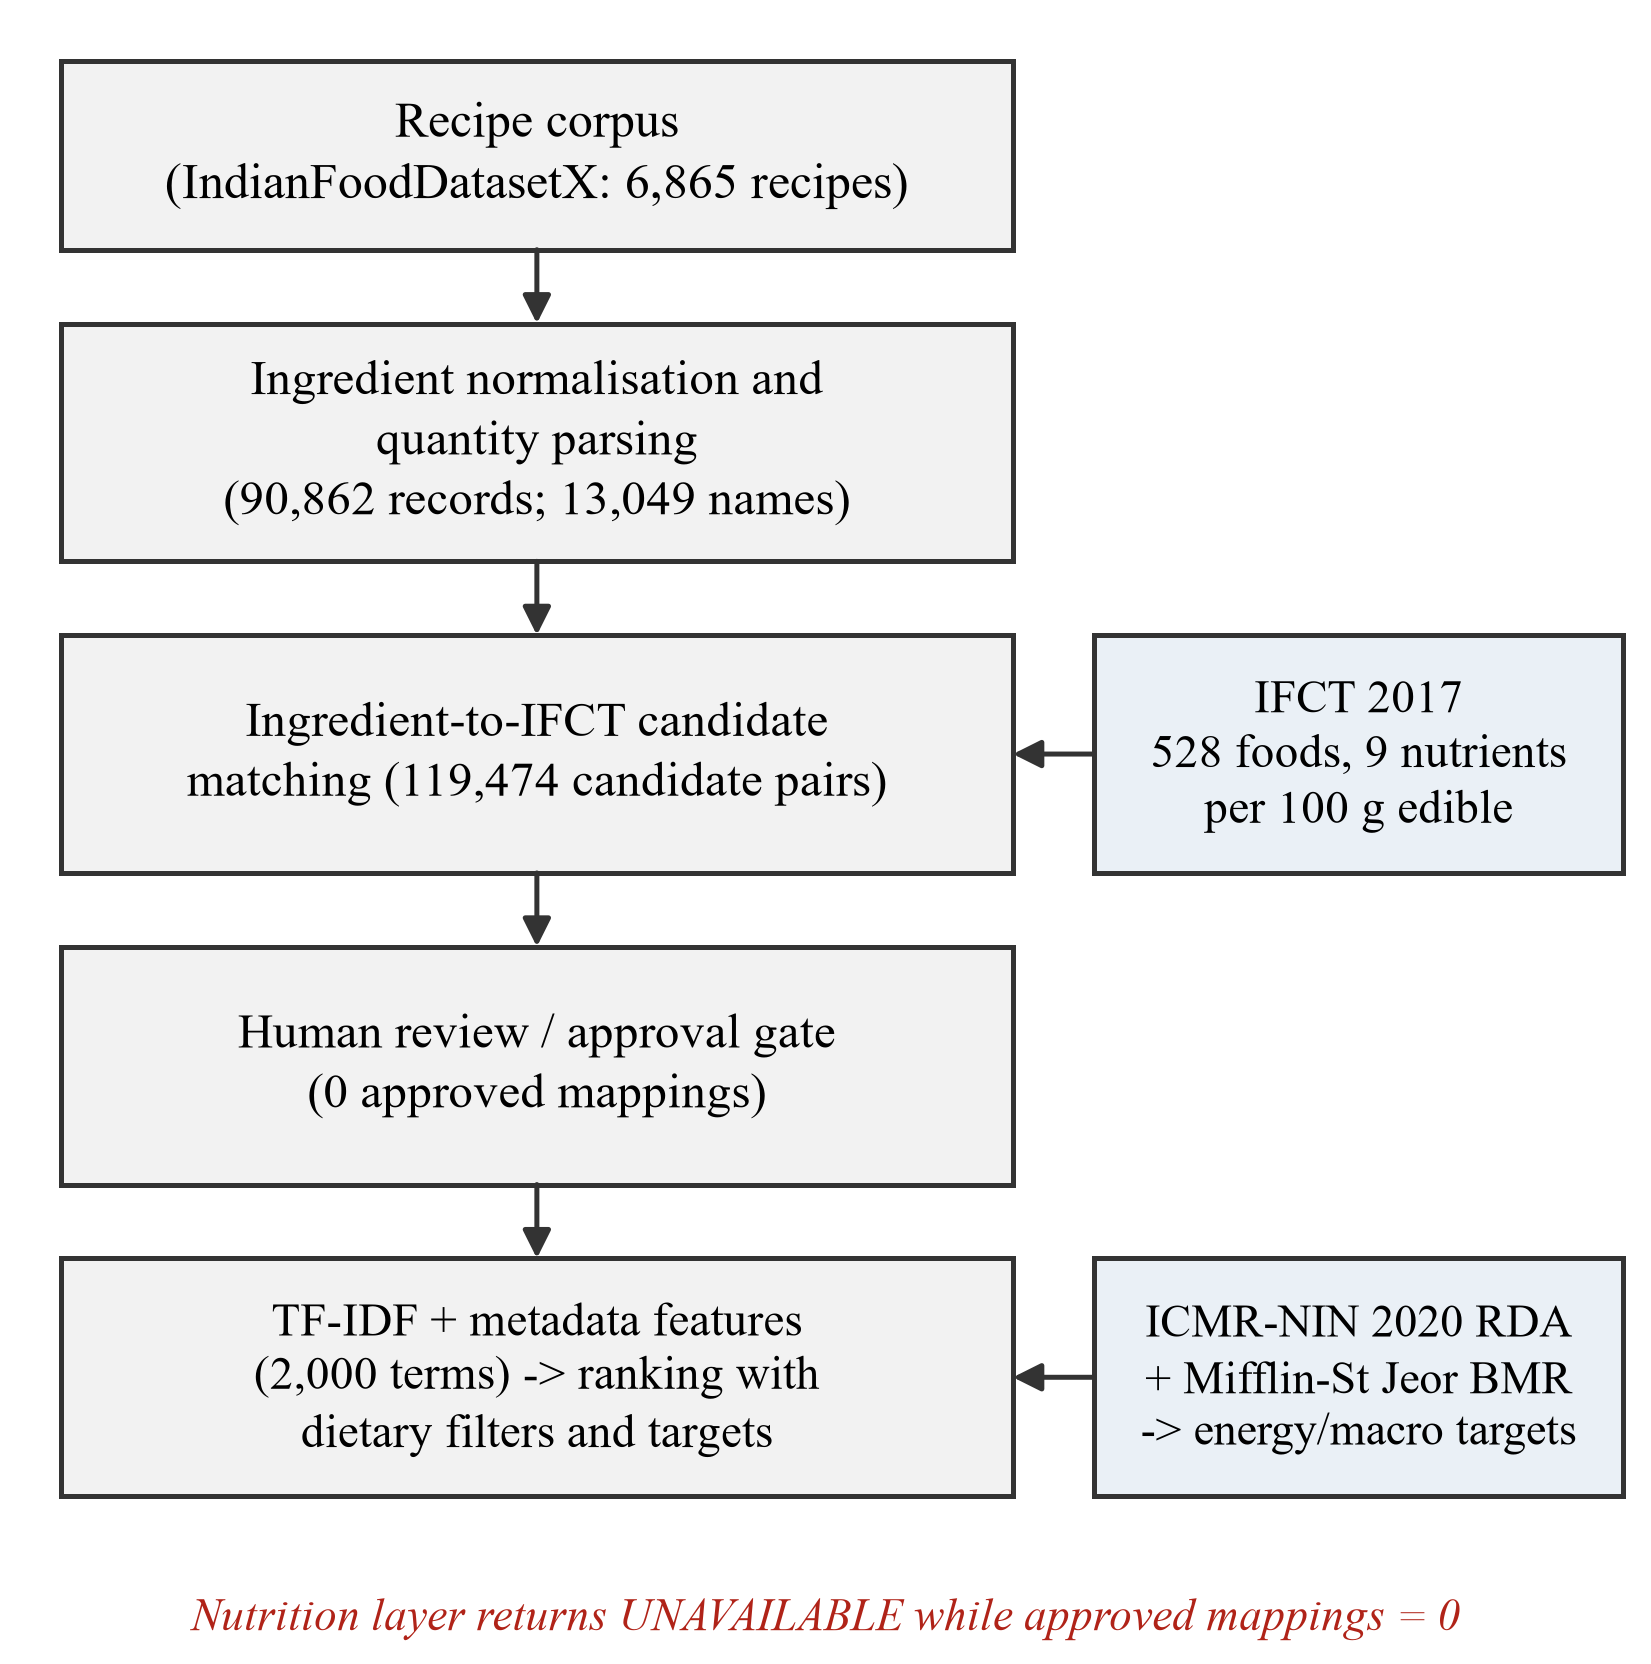
\includegraphics[width=0.92\columnwidth]{figures/fig1_architecture.png}
\caption{System architecture. Recipe text is parsed and matched to IFCT food
codes; only approved mappings may enter the nutrient calculation. The nutrition
layer currently returns an unavailable status because the approval gate has
admitted no mappings.}
\label{fig:arch}
\end{figure}

\subsection{Feature representation and ranking}
\label{sec:features}

Each recipe is represented by (i) a TF-IDF vector over its normalised ingredient
list (2{,}000 features, unigrams and bigrams, minimum document frequency 2,
maximum document frequency 0.95, L2-normalised), and (ii) one-hot cuisine (75 values),
one-hot course (10 values) and multi-label diet (20 labels) encodings. The
similarity between a query recipe $q$ and a candidate $c$ is
\begin{equation}
\label{eq:score}
S(q,c) = 0.4\,J + 0.3\,C + 0.15\,K + 0.15\,D ,
\end{equation}
where $J$, $C$, $K$ and $D$ are computed on $(q,c)$: $J$ is ingredient Jaccard
overlap, $C$ and $K$ are indicator matches on cuisine and course, and $D$ is
diet-label overlap. Dietary constraints (vegetarian,
vegan, eggetarian, Jain, allergen and ingredient exclusions) are applied as hard
filters before ranking, so a constraint-violating recipe is never returned. The
personalisation layer combines the recommendation score with nutrition match,
dietary compliance, meal-slot suitability and stated preference; because nutrition
values are unavailable, the nutrition term is inert and the layer reduces to
similarity plus metadata agreement. Energy targets use Mifflin--St~Jeor basal
metabolism \cite{mifflin1990} multiplied by an ICMR-NIN physical-activity level,
with a $\pm$500\,kcal adjustment for weight goals and protein, fat and fibre
targets from the same reference \cite{icmrnin2020}. These targets are arithmetic on
user input; they have not been clinically validated.

\section{Experimental Setup}
\label{sec:setup}

\emph{Environment.} Experiments ran on a single Windows laptop (no GPU) with
Python 3.15.2, scikit-learn 1.9.1, NumPy 2.5.4, pandas 3.1.1 and SciPy 1.18.1. The
same pipeline is served by a FastAPI backend with a relational store and a React
client; the web layer is not evaluated here.

\emph{Splits.} Recipes are split 70/15/15, stratified by cuisine with seed 42 and a
minimum of five recipes per stratum. Categories with fewer recipes are dropped,
which yields 4{,}783 training, 1{,}025 validation and 1{,}025 test recipes (69.7\%,
14.9\% and 14.9\% of 6{,}865; 32 recipes fall outside the strata) over 63 cuisines.
Splitting is at recipe level, and cross-split checks report zero identifier overlap
and zero near-duplicate pairs at Jaccard $\geq 0.9$. We use the test split only,
with 50 queries sampled from its 1{,}025 recipes; no validation data enter the
reported numbers.

\emph{Proxy relevance.} Without interaction data, a candidate is called relevant
if
\begin{equation}
\label{eq:proxy}
\rho(q,c) = 0.5J + 0.2C + 0.15K + 0.15D \;\geq\; 0.3 ,
\end{equation}
with the component similarities of (2) evaluated on $(q,c)$.
Note that $\rho$ reuses the ingredients of $S$: the proxy rewards exactly the
quantities the rankers optimise, with extra weight on ingredient overlap. Metrics
are Precision@$k$, Recall@$k$, Diversity@$k$ (one minus mean pairwise ingredient
Jaccard inside the list) and Coverage@$k$ (distinct recommended recipes over
catalogue size). All four methods share the query set, the candidate pool and the
query-exclusion rule, and self-recommendation is suppressed.

\emph{Baselines and selection rule.} Random selection with seed 42, a cuisine-match
baseline that restricts candidates to the query cuisine and orders them by $J$, and
a pure-Jaccard ranker are compared with the weighted model of \eqref{eq:score}. The
project fixed deployment thresholds of Precision@5 $\geq 0.20$, Recall@5 $> 0.02$,
Coverage@20 $> 0.50$ and latency $< 500$\,ms, and a composite score
\begin{equation}
\label{eq:composite}
\begin{aligned}
\Phi = {}& 0.30P + 0.20R + 0.15\,\mathrm{Div} + 0.15\,\mathrm{Cov} \\
& + 0.10\left(1 - L/500\right) + 0.10\,\mathrm{Rel},
\end{aligned}
\end{equation}
The reliability term $\mathrm{Rel}$ was never defined or measured in the project;
it is set to 1.0 for all methods, so it shifts every score equally and cannot change
the ranking. We report $\Phi$ only as the project's bookkeeping device.

\section{Results and Discussion}
\label{sec:results}

\begin{figure*}[t]
\centering
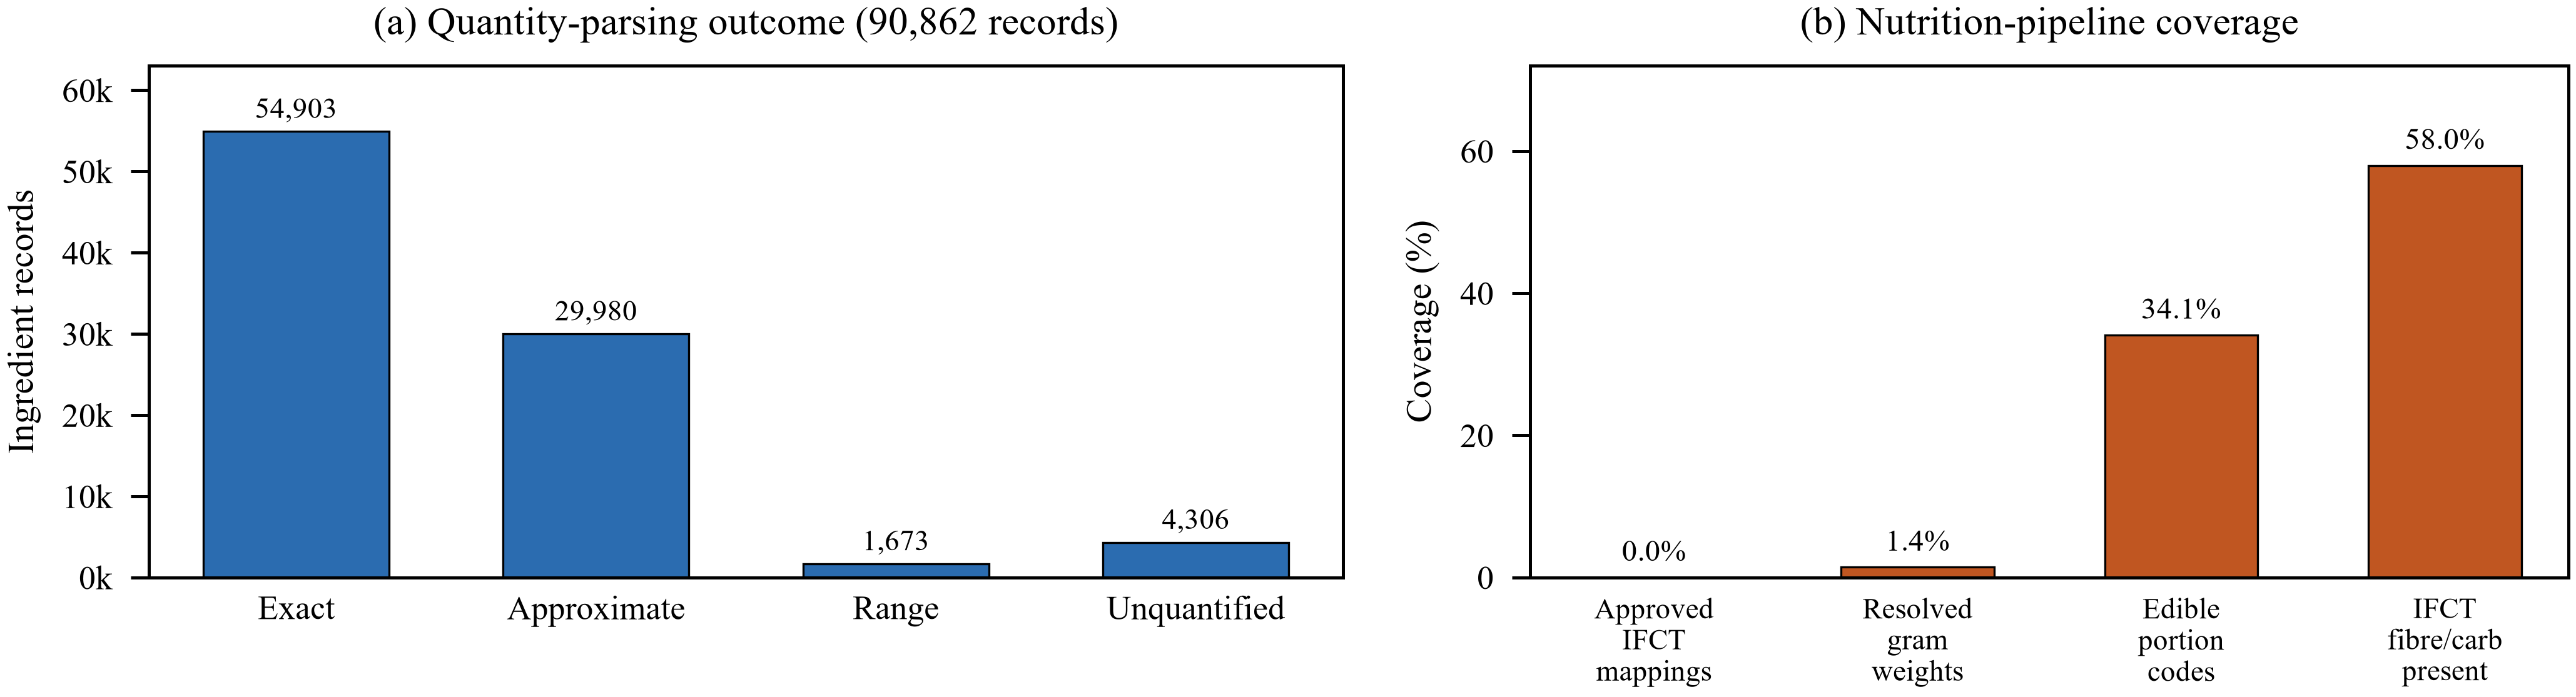
\includegraphics[width=\textwidth]{figures/fig2_pipeline_coverage.png}
\caption{(a) Outcome of quantity parsing over 90{,}862 ingredient rows. (b) Measured
coverage of the four inputs the nutrition engine requires. Only 1.43\% of rows have
a resolved gram weight and no ingredient mapping has been approved, so recipe-level
nutrient totals cannot be computed.}
\label{fig:coverage}
\end{figure*}

\subsection{Recommendation quality}
\label{sec:recresults}

Table~\ref{tab:results} and Figs.~\ref{fig:pr}--\ref{fig:divcov} report the
comparison. The weighted TF-IDF model attains the highest precision (0.996), the
highest proxy recall (0.0157), the second-highest diversity (0.869), coverage of
0.234 and 180\,ms per query. Cuisine match is the strongest baseline on precision
(0.904) and is the only method whose precision degrades gracefully as $k$ grows
(Fig.~\ref{fig:patk}), because its candidate set is restricted to one cuisine.

% Table II -- recommendation results. Source:
% reports/phase5/experiments/results/{baseline,content_based}_experiments.json
% and reports/phase5/stage5_3_2_final_metric_correction.md (composite scores).
\begin{table}[t]
\caption{Recommendation results over the same 50 sampled test queries and the
same 6{,}865-recipe candidate pool. Latency is mean wall-clock time per query.
Composite is the project's weighted score (Section~\ref{sec:setup}); the
reliability term is an unmeasured constant there, so it is not a validated utility.}
\label{tab:results}
\centering
\scriptsize
\setlength{\tabcolsep}{2.6pt}
\begin{tabular}{@{}lcccccc@{}}
\toprule
\textbf{Method} & \textbf{P@5} & \textbf{R@5} & \textbf{Div@10} & \textbf{Cov@20} & \textbf{Lat. (ms)} & \textbf{Comp.} \\
\midrule
Random            & 0.128 & 0.0006 & 0.958 & 0.254 & 110 & 0.182 \\
Cuisine match     & 0.904 & 0.0113 & 0.824 & 0.225 & 390 & 0.441 \\
Jaccard           & 0.548 & 0.0046 & 0.773 & 0.220 & 208 & 0.380 \\
TF-IDF (deployed) & \textbf{0.996} & \textbf{0.0157} & 0.869 & 0.234 & 180 & \textbf{0.595} \\
\bottomrule
\end{tabular}
\end{table}


\begin{figure}[t]
\centering
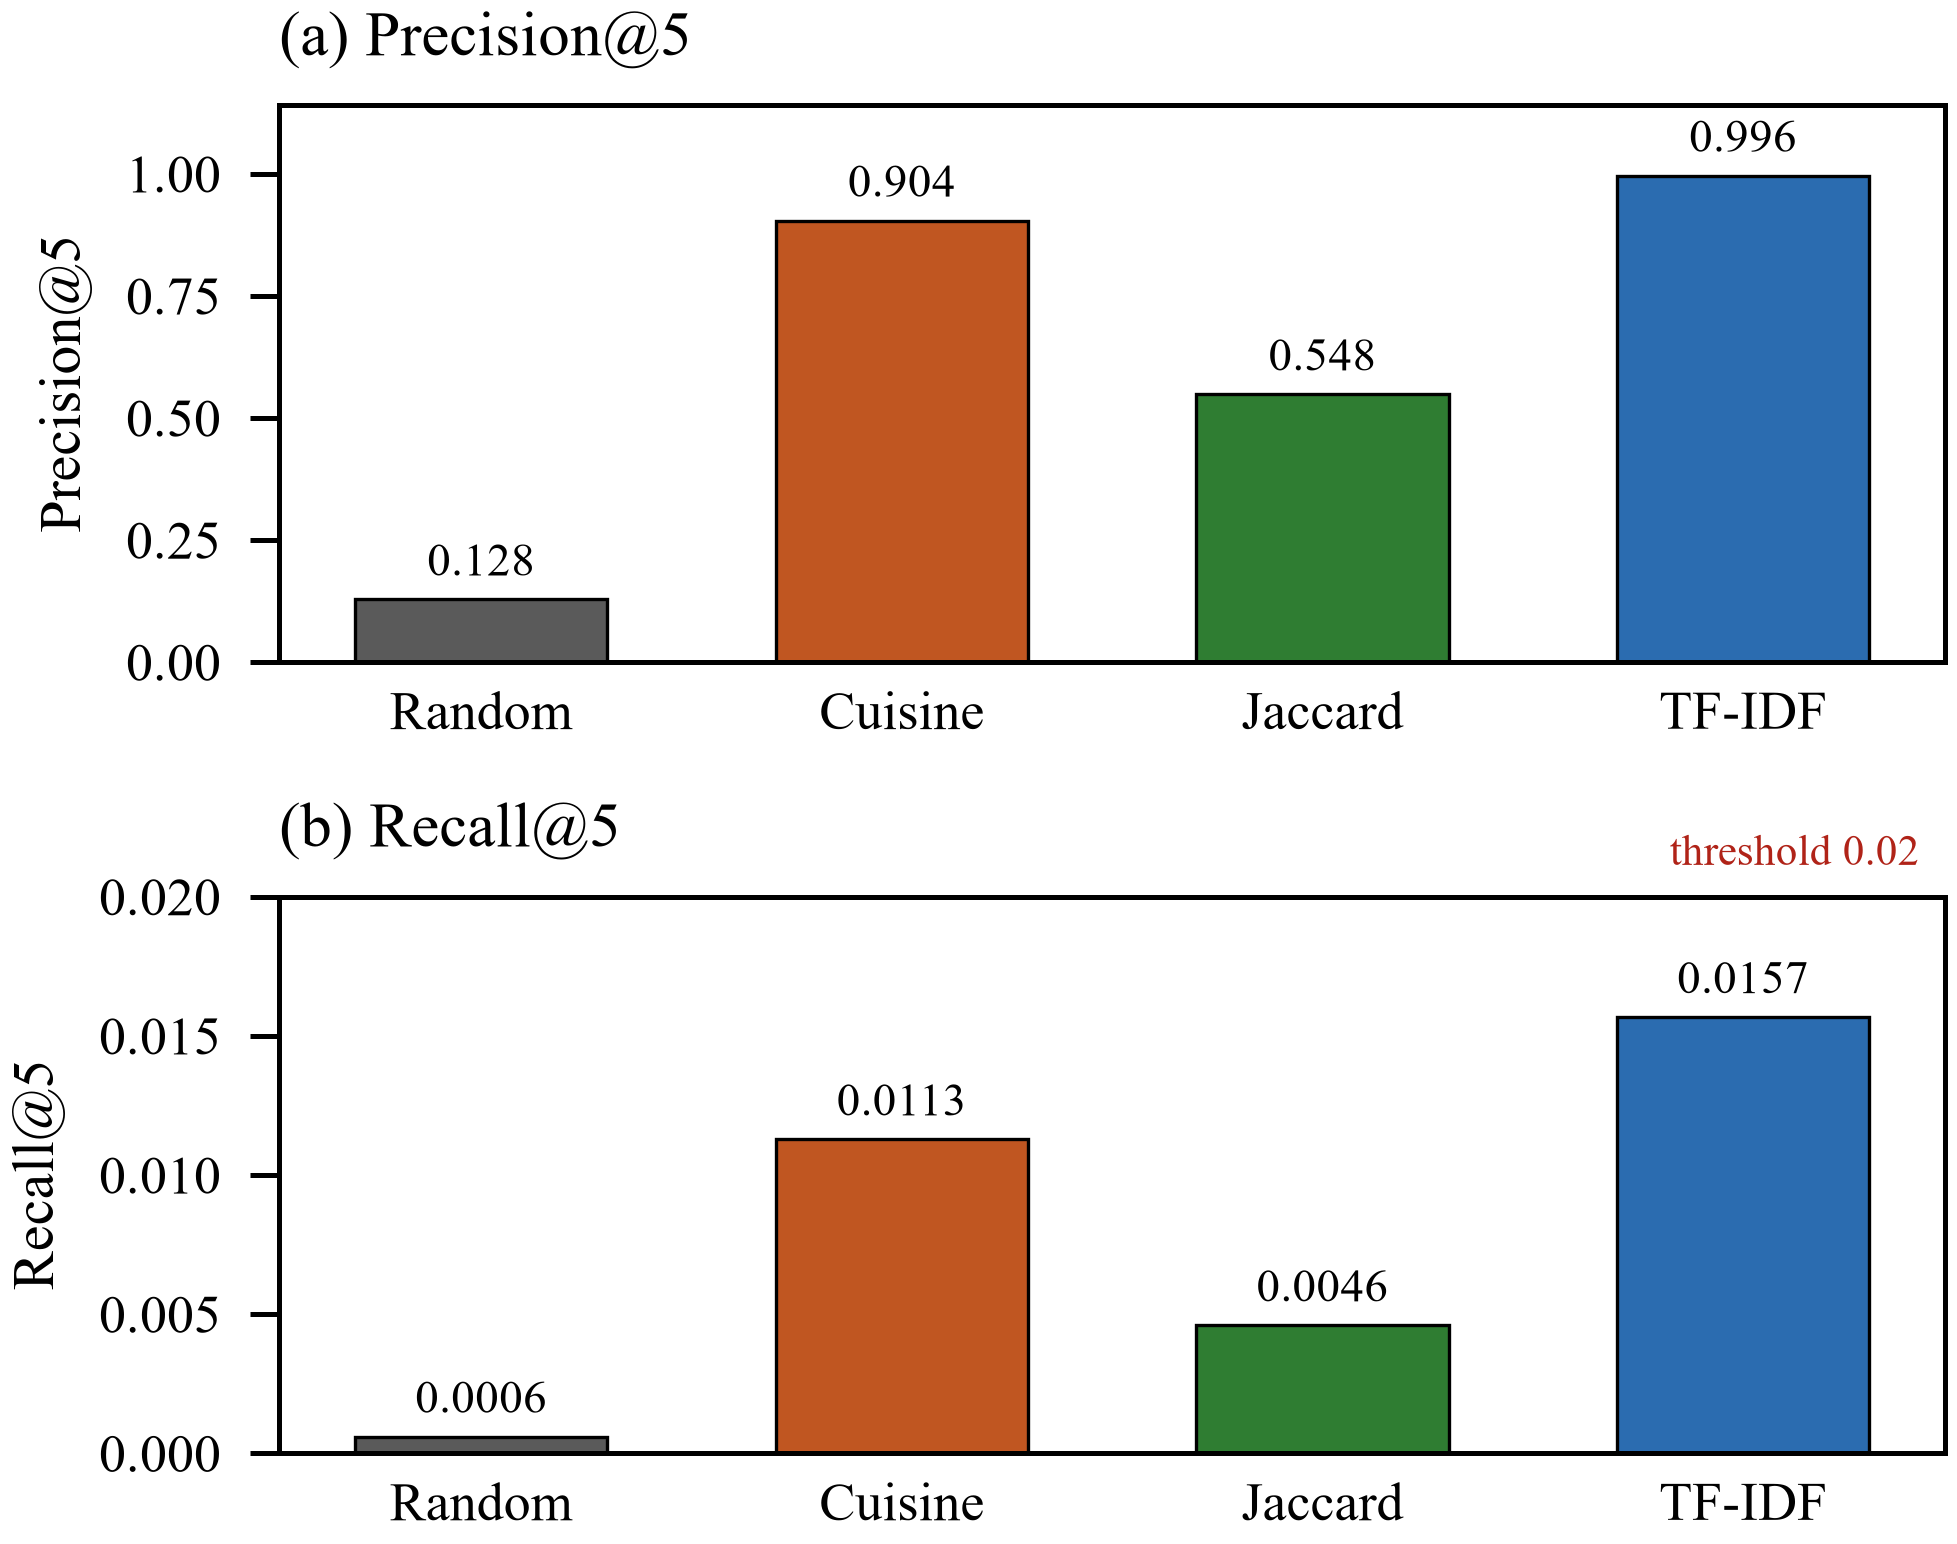
\includegraphics[width=0.92\columnwidth]{figures/fig3_precision_recall.png}
\caption{Precision@5 (a) and Recall@5 (b) on the shared 50-query test sample. The
dashed line marks the project's Recall@5 requirement of 0.02, which no method
meets.}
\label{fig:pr}
\end{figure}

The precision figures must be read carefully. Precision@5 near unity means that
almost every returned recipe clears the proxy threshold of \eqref{eq:proxy}; it
does not mean that the recipes are useful. Three readings are available. First, the
threshold is permissive for same-cuisine, ingredient-overlapping recipes, which is
why a random ranker still collects 0.128. Second, recall is structurally low: with
a threshold that admits many candidates per query, five results can cover only a
small fraction of the relevant set, and the best value observed is 0.0157, i.e.\
roughly one and a half percent. Third, the composite score is driven almost
entirely by the precision term, so a method can win \eqref{eq:composite} while
failing two of the four requirements.

\begin{figure}[t]
\centering
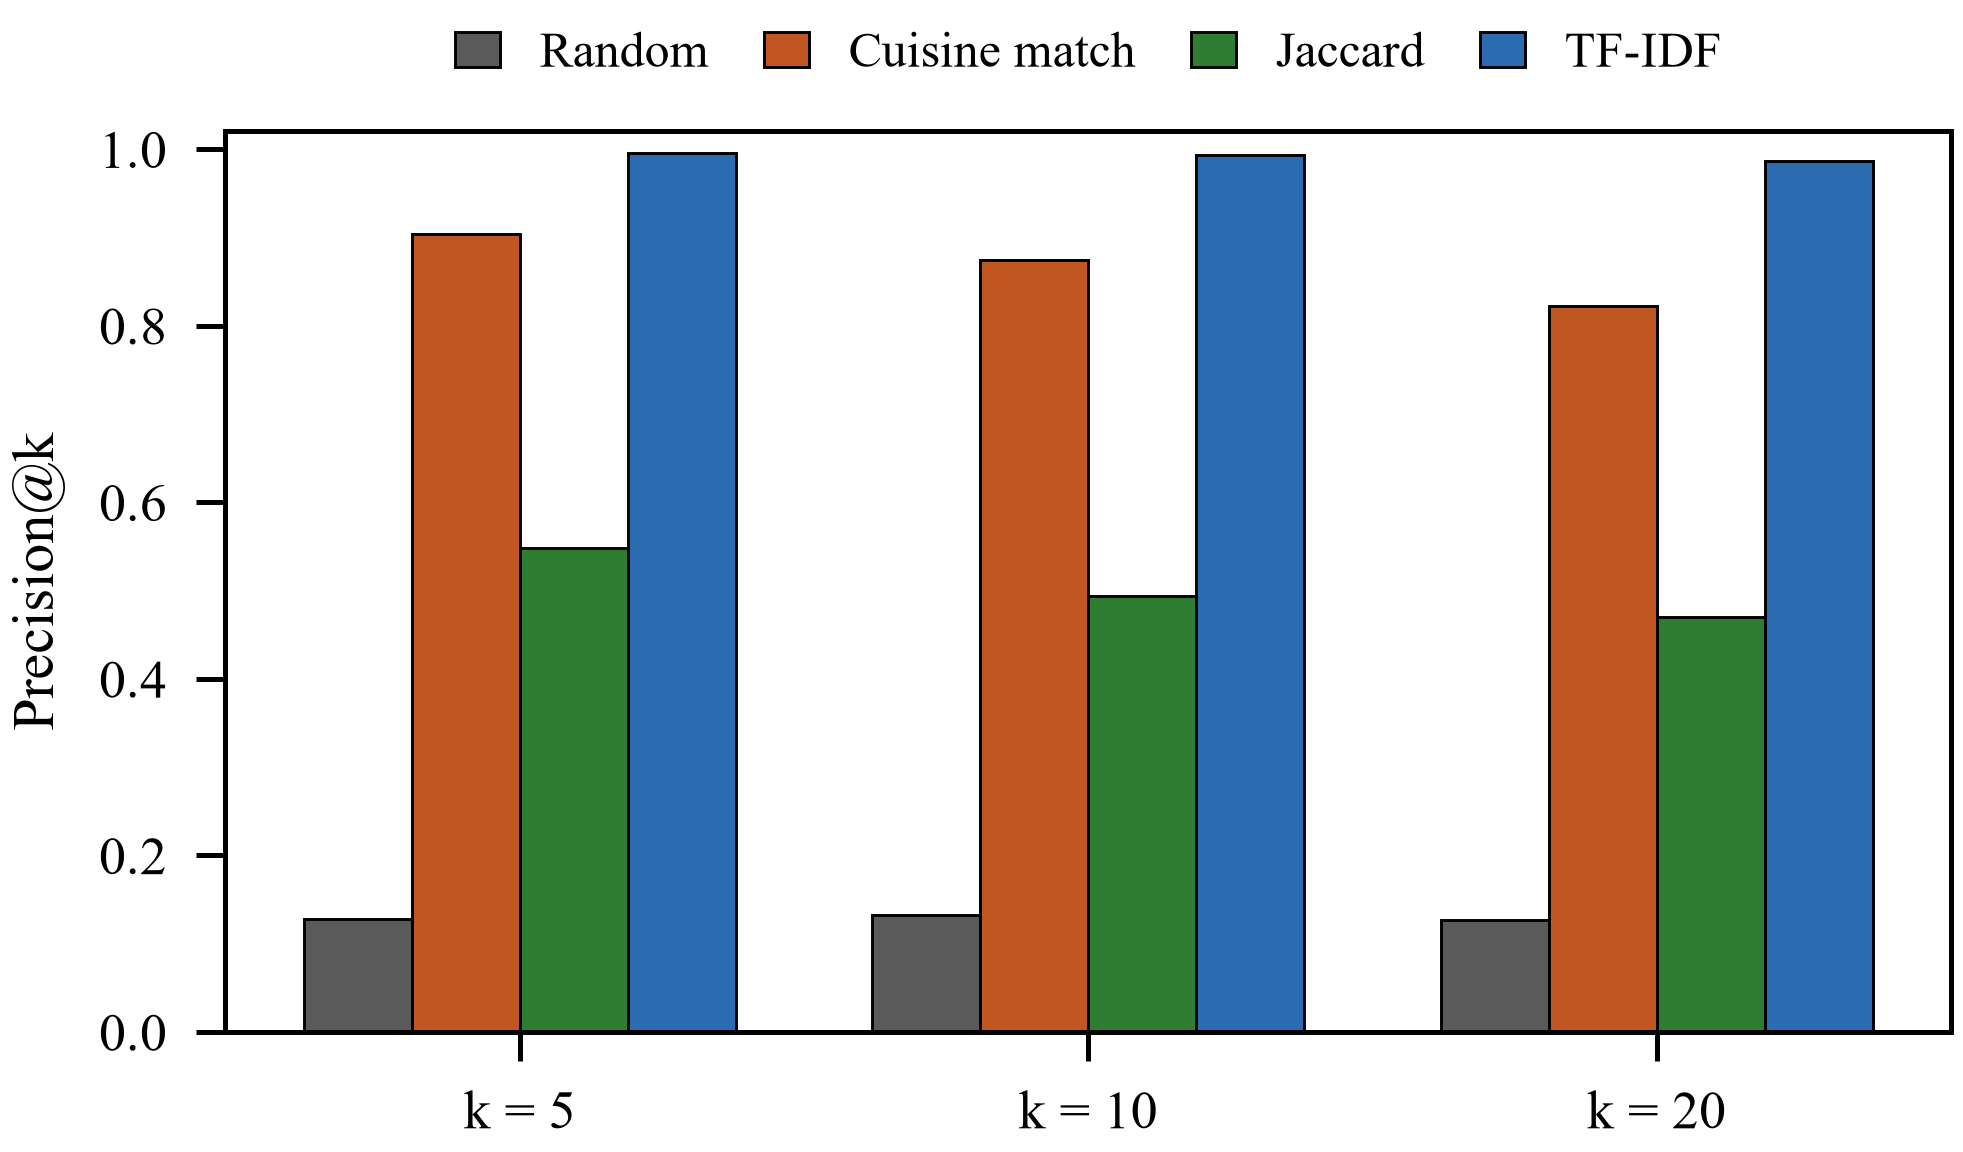
\includegraphics[width=0.92\columnwidth]{figures/fig4_precision_at_k.png}
\caption{Precision as a function of the cut-off. The weighted model is stable
across $k$; the cuisine-match baseline decays from 0.904 to 0.822, and the random
ranker stays near 0.12.}
\label{fig:patk}
\end{figure}

\begin{figure}[t]
\centering
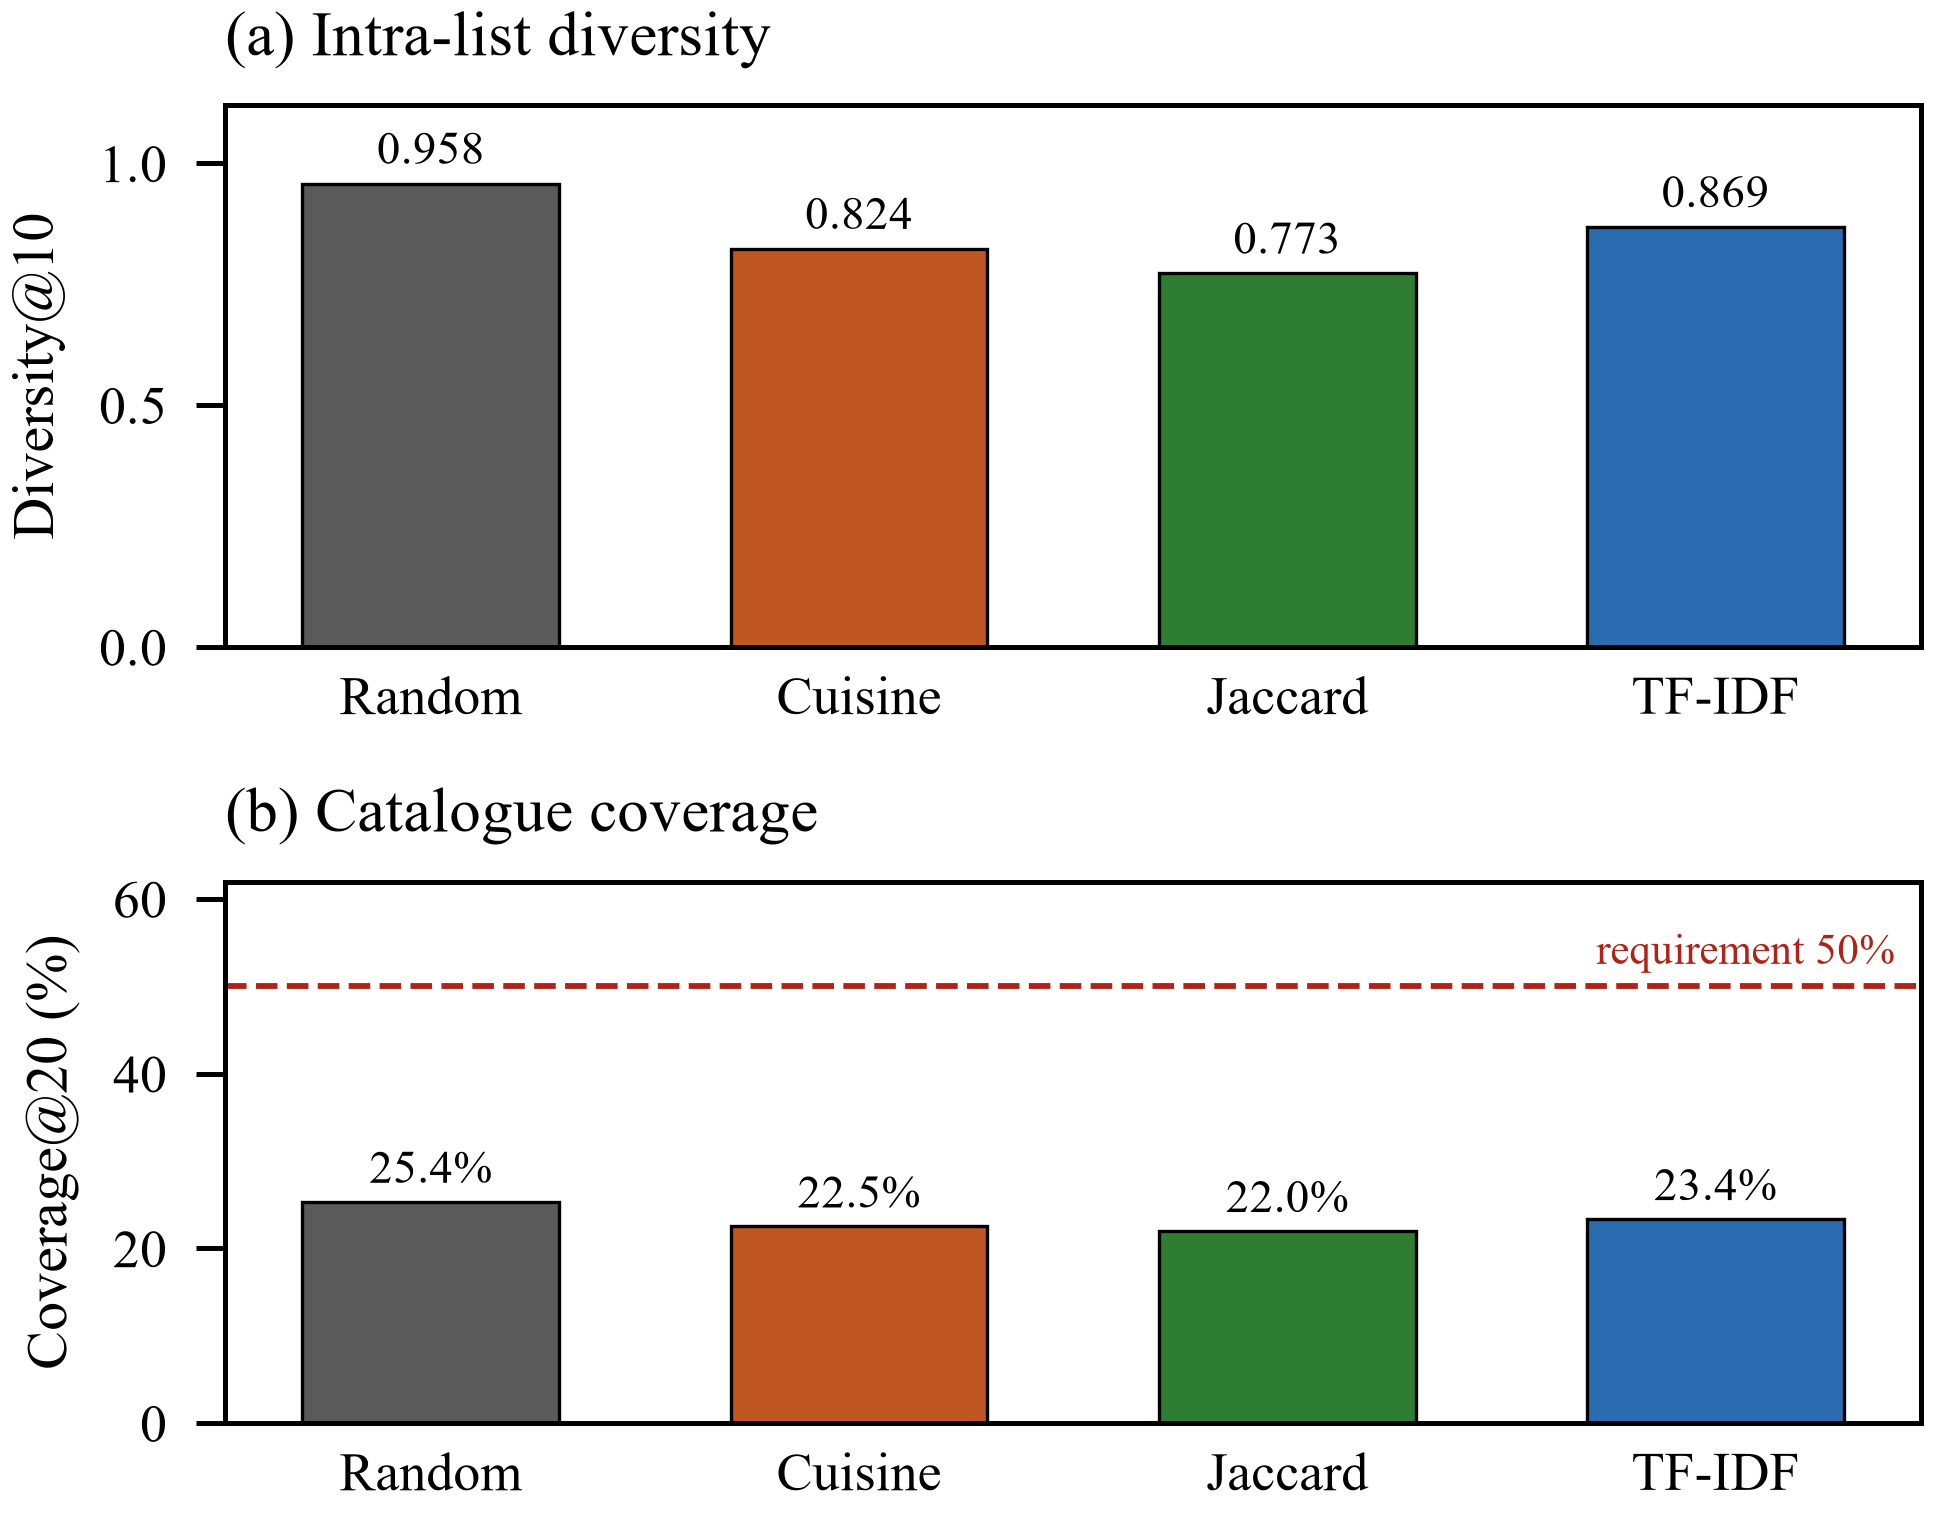
\includegraphics[width=0.92\columnwidth]{figures/fig5_diversity_coverage.png}
\caption{Intra-list diversity (a) and catalogue coverage (b). Coverage is maximal
for the random ranker (25.4\%), which shows that coverage and relevance pull in
opposite directions here; all methods are less than half of the 50\% requirement.}
\label{fig:divcov}
\end{figure}

\subsection{Constraint verification and model selection}
\label{sec:selection}

No method satisfies all four requirements. Precision@5 and latency pass for the
weighted model; Recall@5 (0.0157 against $>0.02$) and Coverage@20 (0.234 against
$>0.50$) fail. The best coverage of any method, 0.254, comes from the random
ranker, and it still falls short by a factor of two. The project therefore deployed
the weighted TF-IDF model on the grounds of highest composite score and acceptable
latency, with the two failures recorded rather than waived. Excluding the undefined
reliability term from \eqref{eq:composite} subtracts 0.10 from every score (0.495,
0.341, 0.280 and 0.082) and leaves the ordering unchanged, so the selection is not
an artefact of that term.

One negative result deserves recording. The content-based experiments were run
under four nominal weight configurations (ingredient-only, equal, ingredient-
focused, metadata-focused), but all four produced numerically identical metrics.
Inspection of the retrieval code showed that the ranker used fixed weights
(0.4/0.3/0.15/0.15) and ignored the configuration object. The apparent agreement
across configurations is therefore a software defect, not evidence that the weights
are insensitive, and we report a single configuration for the weighted model rather
than four.

\subsection{Clustering}
\label{sec:clustering}

Table~\ref{tab:clustering} reports clustering on the combined feature matrix
reduced to 20 principal components. The best silhouette, 0.047 at $K=50$, and the
best Davies--Bouldin index, 3.187 at $K=100$, both indicate weak structure
\cite{rousseeuw1987}. Cluster sizes are strongly skewed and the composition is
dominated by cuisine metadata rather than ingredient patterns. We conclude that
clustering is unsuitable as a primary recommendation mechanism; at most it could
serve as a candidate filter, which we have not evaluated.

% Table III -- clustering. Source: reports/phase5/experiments/results/clustering_experiments.json
\begin{table}[t]
\caption{Clustering on the 6{,}865$\times$595 combined feature matrix reduced to
20 principal components (K-Means and agglomerative, seed 42). All silhouettes are
below 0.05, i.e.\ no configuration yields well-separated clusters.}
\label{tab:clustering}
\centering
\footnotesize
\setlength{\tabcolsep}{4.5pt}
\begin{tabular}{@{}llccc@{}}
\toprule
\textbf{Algorithm} & \textbf{$K$} & \textbf{Silhouette} & \textbf{Davies--Bouldin} & \textbf{Largest cluster} \\
\midrule
K-Means        & 20  & 0.0388 & 4.111 & 655 \\
K-Means        & 50  & \textbf{0.0469} & 3.603 & 287 \\
K-Means        & 100 & 0.0414 & \textbf{3.187} & 201 \\
Agglomerative  & 20  & 0.0172 & 4.214 & 1{,}516 \\
Agglomerative  & 50  & 0.0244 & 3.605 & 613 \\
\bottomrule
\end{tabular}
\end{table}


\subsection{Why the proxy flatters the rankers}
\label{sec:bias}

Equation~\eqref{eq:proxy} gives 50\% of its weight to ingredient Jaccard and 20\% to
cuisine match. The cuisine-match baseline optimises precisely the cuisine
component, and the weighted model optimises all four components, so both are scored
by a function they are built to satisfy. The circularity is not incidental to the
numbers: it explains why precision is near ceiling and why the ordering of methods
is stable under changes of $k$. The error analysis of the project corroborates the
reading. Across 20 inspected queries, 47 recommended items crossed a cuisine
boundary and 16 queries contained generic terms (salt, oil, water, pepper) that
carry little discriminative signal; all three methods disagreed on the top result
for every query. A proxy that rewards shared pantry staples will call such overlaps
relevant.

\subsection{The nutrition layer}
\label{sec:nutrresults}

Fig.~\ref{fig:coverage}(b) is the quantitative summary of the nutrition result:
zero approved mappings, 1.43\% of ingredient rows with a resolved mass, edible
portion factors for 34.1\% of IFCT codes, and fibre and available carbohydrate
present for 306 of 528 foods (58.0\%; the remaining 42.0\% are missing, not zero).
Preparation state is unspecified for 88.6\% of rows, which matters because IFCT
values describe raw foods while recipes describe cooked dishes. Each of these is
individually sufficient to block a defensible recipe-level total, and they compound:
the mapping gate must open before mass coverage becomes the limiting factor. The
engine's behaviour in this state is specified and tested (42 unit tests, including
synthetic fixtures with known answers), and its abstention is deliberate. We regard
that abstention, and the fact that the application displays an unavailable status
rather than zeros, as a substantive result: a system that reports neither partial
sums nor imputed values is more useful to a dietitian than one that reports a
confident wrong number.

\subsection{Limitations}
\label{sec:limits}

The evaluation uses 50 queries from a single corpus, with a proxy that shares
features with the models it scores; it therefore supports comparisons among these
methods only. No human relevance judgements, no user study and no clinical
assessment were performed, and no interaction data exist, which rules out
collaborative filtering. The corpus is scraped, has no explicit licence and mixes
regional naming conventions. Nutrient accuracy is untested for the same reason the
engine abstains. The nutrition-target arithmetic inherits the assumptions of
\cite{mifflin1990} and \cite{icmrnin2020} and has not been checked against measured
energy expenditure. Finally, clustering and weight sensitivity remain open: the
configuration defect noted above means the weighting was never genuinely varied.

\section{Conclusion}
\label{sec:conclusion}

We described a content-based pipeline for personalised Indian meal recommendation
that combines ingredient-level TF-IDF features with cuisine, course and diet
metadata, applies dietary constraints as hard filters, and derives energy and
macronutrient targets from user anthropometry and Indian reference intakes. On 50
sampled test queries the weighted model reaches Precision@5 of 0.996, Recall@5 of
0.0157, Diversity@10 of 0.869, Coverage@20 of 0.234 and 180\,ms per query, and
scores highest on the project's composite measure; it nevertheless fails the
project's recall and coverage requirements, as does every other method tested.
Clustering offers no usable structure (best silhouette 0.047). The nutrition
component cannot be validated at all in the current state, because the corpus has
no approved ingredient-to-IFCT mappings and only 1.43\% of ingredient rows carry a
resolved mass, and the engine consequently abstains.

The honest summary is a working recommendation and planning component evaluated
under a biased proxy, attached to a nutrition component that is implemented, tested
and deliberately silent. Closing the gap requires work that is organisational as
much as technical: complete a reviewed mapping of high-frequency ingredients,
expand household-measure and piece-weight coverage, and collect genuine relevance
judgements so that precision and recall can be measured against people rather than
against a function of the features themselves.

\balance
\bibliographystyle{IEEEtran}
\bibliography{references}

\end{document}
